\section{Narzędzia wspomagające}
\label{narzedzia}

\begin{frame}
    \frametitle{Rodzaje narzędzi wspomagających}
    \begin{itemize}
        \item systemy kontroli wersji
        \item planowanie zadań
        \item komunikatory internetowe
    \end{itemize}
\end{frame}

\begin{frame}
    \metroset{block=fill}
    \frametitle{Systemy kontroli wersji}
    \begin{block}{Definicja}
        System kontroli wersji to oprogramowanie służące do śledzenia zmian 
        w kodzie źródłowym oraz pomocy w łączeniu zmian dokonanych w plikach przez 
        wiele osób w różnym czasie.
    \end{block}
\end{frame}

\begin{frame}
    \frametitle{Systemy kontroli wersji}
    \begin{itemize}
        \item git
        \item subversion
        \item mercurial
    \end{itemize}
\end{frame}

\begin{frame}
    \frametitle{Systemy kontroli wersji}
    \vspace{-0.5cm}
    \begin{figure}
        \leftskip-0.3cm
        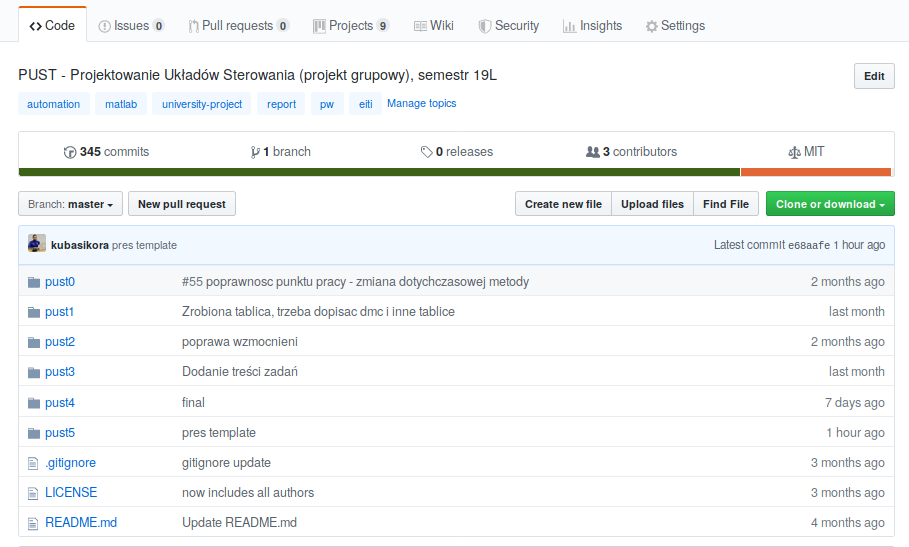
\includegraphics[scale=0.35]{./images/git_example.png}
        \caption{Zrzut ekranu z repozytorium w serwisie \texttt{github.com}}
    \end{figure}
\end{frame}

\begin{frame}
    \frametitle{Planowanie zadań}
    \metroset{block=fill}
    \begin{block}{Wymagania względem systemu planowania}
        Powinien być dostępny on-line i umożliwiać podział zadań na trzy grupy:
        \begin{itemize}
            \item do zrobienia,
            \item wykonywane,
            \item zakończone.
        \end{itemize}
    \end{block}
\end{frame}

\begin{frame}
    \frametitle{Aplikacje wspomagające planowanie zadań}
    \begin{itemize}
        \item trello
        \item github
        \item asana
    \end{itemize}
\end{frame}

\begin{frame}
    \frametitle{Aplikacje wspomagające planowanie zadań}
    \begin{figure}
        \centering
        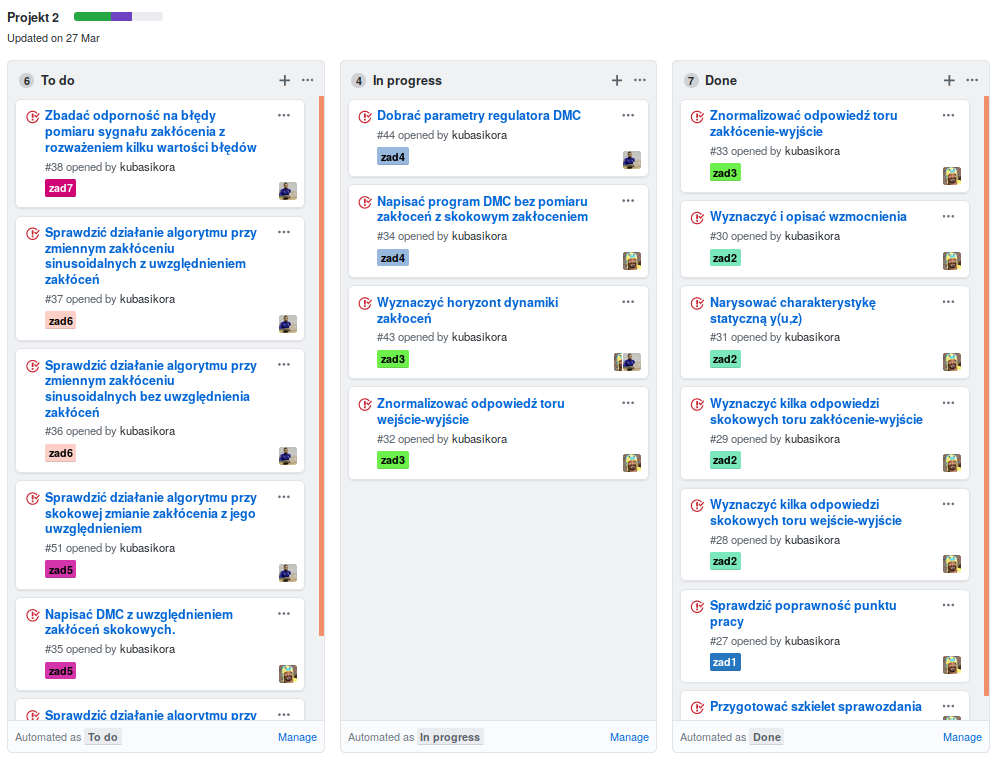
\includegraphics[scale=0.26]{./images/github_example.png}
        \caption{Zrzut ekranu z listy zadań w serwisie \texttt{github.com}}
    \end{figure}
\end{frame}

\begin{frame}
    \frametitle{Komunikacja przez internet}
    \begin{itemize}
        \item messenger
        \item slack
        \item e-mail
    \end{itemize}
\end{frame}

\begin{frame}
    \frametitle{Komunikacja przez internet}
    \begin{figure}
        \centering
        
\includegraphics[scale=0.3]{./images/messenger_example.png}
        \caption{Zrzut ekranu z konwersacji grupowej}
    \end{figure}
\end{frame}


